\documentclass{article}
\usepackage[a4paper, total={6in, 8in}]{geometry}  
\usepackage{graphicx} % pour insérer des images
\usepackage{hyperref} % pour insérer des liens

% pour utiliser des notations scientifiques
%\usepackage{amssymb}
%\usepackage{amsmath}
%\usepackage{amsfonts}

%\usepackage{extarrows} % pour afficher les flèches de logiques (implique, équivalent à ,etc...)
%\usepackage{soul} % utilité à troiver
%\let\oldemptyset\emptyset
%\usepackage[T1]{fontenc}

\author{Amnézic}
\date{2024}
\title{Aide Vancouver}

\begin{document}
\maketitle
\newpage
\tableofcontents
\newpage

\section{Introduction}
Ce document n'est pas un document officiel, c'est juste un document que j'ai écrit pour résumer un peu comment se passe le semestre à l'étranger à Vancouver. Mon année est la première année à faire un partenariat avec BCIT Vancouver donc il se peut que certaines choses changent mais je pense que la grande majorité des informations resteront identiques d'une année sur l'autre.\newline
Ce document est une aide qui va servir pour les années suivantes et pourra toujours être complétée, je mettrai le document .tex pour que ceux qui veulent puisse l'éditer. Pour la première édition de ce document, ce sera principalement de l'expérience personnelle et un peu des autres épitéens qui viennent avec moi, donc je m'exprimerai souvent à la première personne du singulier ou du pluriel.\newline
Nous sommes 7 à partir à Vancouver en 2024 (donc nous sommes de la promo 2027), je mettrai leur nom prénom et leur pseudo Discord si jamais il y a besoin. Ce document est là justement pour que toutes les petites astuces que l'on trouve là bas ne se perdent pas et qu'elles puissent être consultées à n'importe quel moment. Si jamais ce document n'est toujours pas actualisé après quelques années, il sera probablement inutile de nous contacter : la mémoire humaine n'est pas immuable.\newline
Je vais diviser ce document en au moins 3 grandes parties : avant le départ, pendant le S4 et après le S4. Cependant, comme il y aura très peu à dire sur la première et la dernière partie, cela pourra être modifiée par la suite.\newline\newline

Je parlerai en dollar mais ce ne sont pas des dollars américains mais des dollars canadiens. À l'heure où j'écris ce texte, un € revient à peu près 1,5 dollar canadien. Un conseil, avant votre départ au Canada, allez échanger un peu d'argent à un bureau de change \textbf{pas à l'aéroport} car les commissions y sont beaucoup plus avantageuses : entre 15 et 20\% dans les aéroports contre quelques pourcents seulement ailleurs.

\section{Avant le départ}
Tout d'abord, félicitations pour avoir été sélectionné pour aller à BCIT. Nous avons pas beaucoup à faire avec EPITA ou BCIT pour la préparation du semestre à l'étranger : EPITA a fait appel à une entreprise tierce qui s'appelle Studies'up il me semble (À VÉRIFIER). Une personne qui travaille là-bas, Camille, nous a aidé et guidé dans tous ce qui était démarche administratives et étudiants avec BCIT. L'année commence assez tôt (début janvier) donc nous avons été amené à faire toutes les démarches dans un intervalle de temps assez restreint (il me semble qu'on a commencé vers mi-octobre). Je ne sais plus l'ordre exact dans lequel on a fait les papiers mais plus ils sont fait vite mieux c'est.\newline
Si jamais une de mes indications vous semble incorrecte ou étrange, n'hésitez pas à aller vérifier l'info par vous même sur internet ou à la personne qui se charge de vous dans les démarches administratives.
\subsection{Le logement}
Il faut savoir que le loyer à Vancouver est, pour une raison encore inconnue, très élevé, il n'est donc pas simple de se loger sans trop dépenser. Il y a plusieurs moyens de se loger à Vancouver:
\begin{itemize}
    \item les chambres étudiantes de BCIT
    \item les appartements étudiants de GEC
    \item le logement chez l'habitant
\end{itemize}
\noindent\textbf{Les chambres étudiantes de BCIT :}\newline
Je vais être très court sur cette partie car nous n'avons pas pu y avoir de place, les résidences étant déjà remplies avant que nous soyons acceptés à BCIT. Ce retard peut être dû au fait que c'est la première année que l'EPITA propose à  Vancouver et que tout ça se soit fait un peu à la dernière minute.\newline\newline 

\noindent\textbf{Les appartements étudiants de GEC :}\newline
Bien que BCIT n'ait pas pu nous proposé des chambres étudiantes sur leur campus, ils nous ont proposé de loger dans un groupe de résidences étudiantes avec qui ils ont un partenariat : GEC. N'ayant pas pris cette option, je vais décrire l'expérience qu'a vécu Shreya dans ces appartements.\newline
(Demander des informations à Clovis)\newline\newline
\noindent\textbf{Le logement chez l'habitant :}\newline
Selon moi, l'option précédente était trop onéreuse et les résidences étaient trop éloignées du campus. J'ai donc choisi cette dernière option : le logement chea l'habitant. Pour ceux qui ne connaissent pas le concept : ce sont des personnes qui habitent là toute l'année mais qui louent les chambres qu'ils ont de disponible chez eux. Les deux principales plateformes pour chercher un logement chez l'habitant :
\begin{itemize}
    \item \href{https://www.homestay.com/fr}{Homestay}
    \item \href{https://www.homstayin.com/fr}{Homestayin}
\end{itemize}
Il n'y a pas un des sites que je vous recommande plus qu'un autre. Lors de votre choix, il faut bien faire attention cependant car certaines annonces affichent le prix par semaine et d'autres par mois. De plus, certaines personnes incluent le budget nourriture tandis que d'autres non. Donc soyez vigilant sur toutes les options pour les différents choix que vous faites.\newline\newline\newline

De manière générale, il n'y a pas de bons ou mauvais endroit ou habiter mais si je peux vous donner un conseil c'est d'habiter dans Vancouver, pas forcément Downtown, si possible le centre ou l'est. Mieux vaut ne pas aller à l'est de Burnaby ou dans Vancouver ouest et nord, car il y aura beaucoup de transports sinon. Certains cours peuvent commencer à partir 8h30 et finir jusqu'à 21h30. Regardez bien s'il y a au moins un ou deux arrêts de bus à côté de là où vous voulez loger.


\subsection{Papiers administratifs et cie}
Cette partie sera un peu barbante mais elle est malheureusement nécessaire. Pour votre départ, il sera nécessaire :
\begin{itemize}
    \item la lettre d'admission de BCIT : elle contiendra certaines informations telles que les dates de début/fin de semestre, le prix et information pour le virement. Elle vous sera demandé pour l'obtention de votre VISA. Un conseil, payez la fac dès que possible, ça fera quelque chose de moins à penser et permettra de régler les problèmes s'il y en a. Camille ou celle qui s'occupera de vous vous dira sûrement que le paiment peut prendre plusieurs semaines mais il ne mettra en réalité qu'à peu près une semaine au grand maximum, c'est-à-dire pour ceux qui sont de toutes petites banques.
    \item une assurance rapatriement
    \item une assurance maladie/mutuelle \textbf{qui peut être utilisé au Canada}; une attestation de la sécurité sociale n'est pas valable au Canada. Si vous n'en avez pas, il vous sera peut être proposé Chapka qui est valable au Canada et qui coûte à peu près 248 €.
    \item VISA/Student permit
\end{itemize}

Pour aller au Canada, il est obligatoire d'avoir un visa ou un student permit. Ils permettent tous les deux de voyager au Canada et d'y rester pendant une durée limitée. La seule différence est que le student permit permet de pouvoir avoir un petit boulot à côté de la fac. Le visa ne coûte que 7 dollars mais le student permit en coûte 180.\newline
Peu importe que vous preniez le visa ou le student permit, il faudra aller donner ses empreintes au gouvernement canadien. Lorsque vous prendrez votre visa/student permit, il vous sera normalement indiqué la procédure : prendre rendez-vous dans un centre (il n'y a que deux : un à Paris et un à Rennes), le jour venu, s'y rendre avec votre passeport et vos empreintes et une photo de vous seront enregistrées. La prise de photo et des empreintes digitales ne dure pas plus de 5 minutes, 10 minutes maximum en cas de grande affluence ou problème. Une fois tous ces documents en poche, il ne faudra pas oublier de prendre l'AVE (autorisation de voyage électronique) qui vous permettra de prendre l'avion pour le Canada.
Pour tous les papiers reliés aux gouvernement canadiens, il faudra faire les démarches sur le site gu gouvernement canadien (INSÉRER LE LIEN DU SITE). 

\section{Pendant le S4}
Cette section sera bien plus développée que la précédente ou la suivante et permettra à ceux qui liront ce document de connaitre un peu Vancouver avant d'y aller et surtout de ne pas refaire les mêmes erreurs que ceux qui y sont allés les années précédentes. 
\subsection{Les contacts d'urgence à contacter en cas de problème}
\subsection{Payer et les télécommunications}
La plupart des banques en France sont centralisées avec la Banque de France et il est donc possible de payer et retirer partout en France avec n'importe quelle carte bleue. Au Canada comme dans pas mal d'autres pays, il y a une différence entre la carte de crédit et la carte de débit. Je développerai cette différence là dès que je l'aurai un peu mieux comprise. De plus, dès que vous faites un paiement à l'étranger, vous avez une petite taxe en plus, il faut donc une solution pour payer le moins de taxes ou pas du tout dans le meilleur des cas.
La solution la plus simple est d'ouvrir un compte sur des banques en lignes comme Revolut qui propose des cartes bancaires sans frais à l'étranger (à compléter), je n'ai pas pris cette option donc je ne pourrai pour le moment pas en parler. Je ne sais pas si cette carte permet de retirer un certain moment par mois et si oui lequel.\newline
Personnellement, ma banque propose une option qui permet de payer une vingtaine d'€ par mois et de ne pas avoir cette taxe là sur mes achats. Dans tous les cas, il vous faudra trouver une solution car sinon la facture risque d'être salée au retour en France.
\subsection{Se nourrir}
\begin{itemize}
    \item
\end{itemize}
\subsection{Se déplacer}
Pour avoir une idée générale des distances et des temps de transports entre 2 endroits à Vancouver, il est possible d'utiliser CityMapper. Cependant, une fois sur place, la plateforme Translink permet d'avoir les vrais nombres en temps réels.
\subsubsection{Le taxi :}
Cette partie sera très courte car elle ne concernera qu'une minorité de vos déplacements normalement. Je pose ça là surtout pour des voyages comme retour de ou aller à l'aéroport et les déplacements urgents. À Vancouver, il n'y a pas qu'une seule entreprise de taxis comme à Paris, il y en a pleins de petites.\newline
Une chose importante si jamais vous prenez le taxi pour sortir de l'aéroport, les prix sont assez fixes, c'est-à-dire que Vancouver est séparé en plusieurs zones, et chaque zone à son prix. les prix indiqués sur la carte ci-dessous correspondent à ce que vous devrez payer si vous êtes au début de cette zone. Une fois rentré dans la zone, il est rajouté au prix initial un surplus au kilométrage. (cf figure 1)
Pour plus d'informations, vous pouvez vous rendre sur cette page : \href{https://www.yvr.ca/en/passengers/transportation/taxis}{YVR Taxis}.
\subsection{Les transports en commun :}
Dans la vie de tous les jours, il est évident que vous prendrez les transports en commun. Vancouver dispose de 3 lignes de métro et d'innombrables lignes de bus. L'ensemble du réseau de transports en commun eest géré par \href{https://www.translink.ca/}{Translink}, c'est via ce site que vous aurez toutes les informations supplémentaires que vous cherchez.\newline
La ville est divisée en 3 grandes zones :

Malheureusement, il n'y a pas de réductions étudiantes à Vancouver pour les étudiants étrangers.\newline
La plupart des cours se feront sur le campus de Burnaby (3700 Willingdon Ave, Burnaby, BC V5G 3H2) mais certains cours se dérouleront aussi sur le campus Downtown (555 Seymour St, Vancouver, BC V6B 3H6) qui sont tous les deux dans les zones 1/2 donc il est préférable de prendre l'abonnement mensuel 2-zone (\href{https://www.translink.ca/transit-fares/pricing-and-fare-zones}{Prix et zones de Vancouver}), à 140\$ par mois, soit à peu près 95€. Si jamais vous voulez découvrir ce qu'il y a dans la zone 3, il vous suffira de payer la différence du prix du ticket unitaire entre la zone 3 et la zone 2.\newline
(cf figure 2)\newline\newline

Une fois sur place, pour prendre un abonnement, vous pouvez soit vous rendre dans une station de métro soit vous rendre dans un des \href{https://www.translink.ca/-/media/translink/documents/transit-fares/where-to-buy/london_drugs_compass_vending_machine_locations.pdf}{London Drug store de Vancouver}. Attention, la machine ne prend que les espèces (jusqu'au billet de 20\$ inclus).
\begin{itemize}
    \item
\end{itemize}
\subsection{Loisirs et passe-temps}
\begin{itemize}
    \item
\end{itemize}
\subsection{Petits trucs et astuces qui peuvent servir}
\begin{itemize}
    \item les prises électriques ne sont pas les mêmes que dans l'Union €péenne, il vous faudra prendre un adaptateur pour les prises canadiennes qui sont les mêmes que les prises américaines.
    \item n'hésitez pas à vous rendre dans des magasins style Dollar Store ou Dollarama, ce sont des boutiques où tout est à 1 ou 2\$ et où il y a pleins de produits du quotidien qui pourront vous être utile, même si ce n'est pas forcément de la super top qualité comme vous ne resterez que quelques mois.
\end{itemize}
\subsection{Choc culturel}
\begin{itemize}
    \item
\end{itemize}
\section{Après le S4}

\section{Annexe}
\begin{figure}[h]
    \centering
    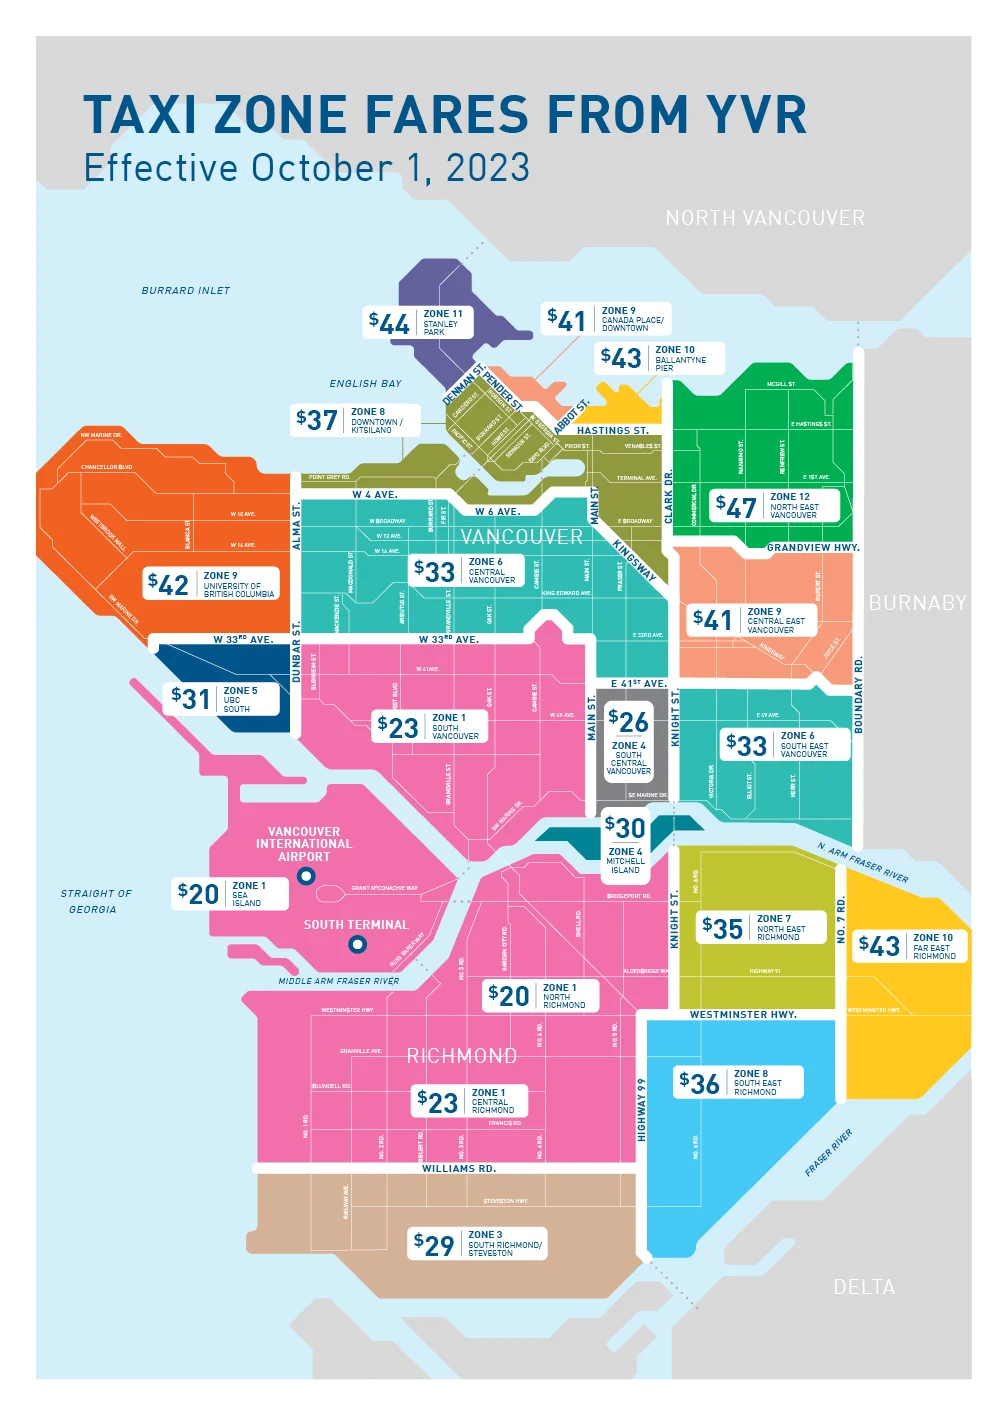
\includegraphics[scale=0.3]{carte_taxis_Vancouver.png}
    \caption{}
\end{figure}

\begin{figure}[h]
    \centering
    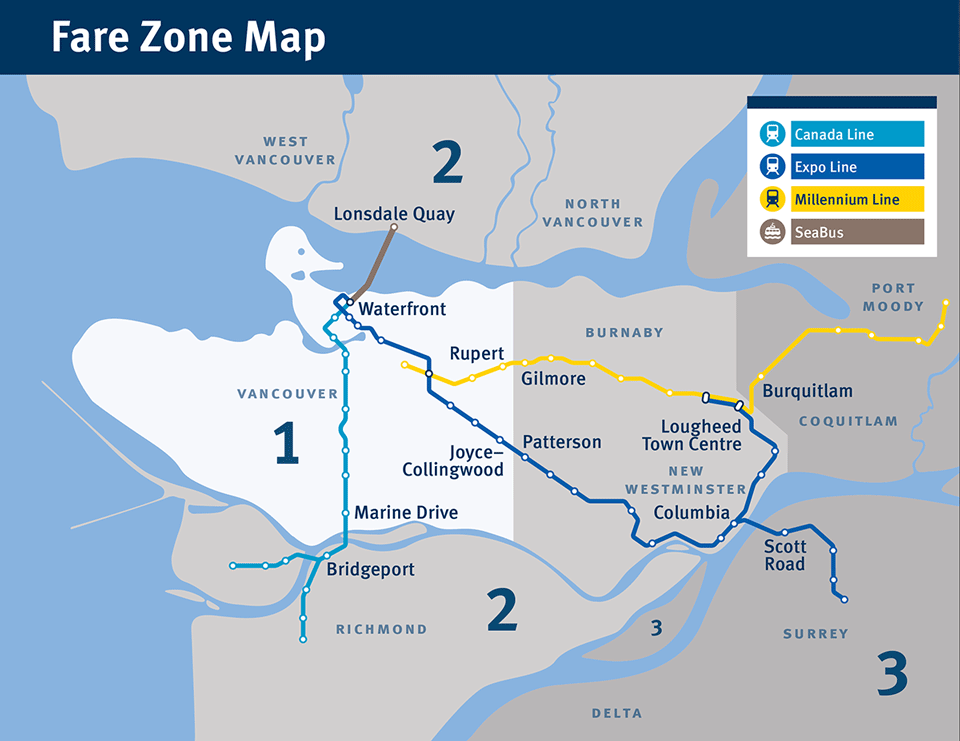
\includegraphics[scale=0.3]{vancouver_sections.png}
    \caption{}
\end{figure}

\end{document}
